\setcounter{section}{-1}
\section{Introduction}

The basis of this lecture course has been the parallelisation of various numerical methods, with a particular focus on the Finite Element Method. For this project we have been supplied with a (subsection of a) software package (which we shall henceforth call \emph{the FEM package}) that computes the solution to the Poisson partial differential equation using the Finite Element Method. This package is self-contained - it includes its own custom matrix/vector types, and its own implementations of linear algebra operations on these types. Our goal is to make improvements to the package with the help of FLENS.

FLENS (\emph{Flexible Library for Efficient Numerical Solutions}) is a C++ library written by Dr. Michael Lehn, which offers a comprehensive collection of matrix and vector types. Included is a C++ -based BLAS (\emph{Basic Linear Algebra Subfunctions} implementation, which provides linear algebra operations, such as matrix-vector multiplication, on these types. 

The advantages of using FLENS in the FEM package are numerous. Firstly, use of an external library for matrix/vector types adds some standardisation to the package, aiding, for example, a user who is new to the FEM package, but has experience of FLENS from other projects. Secondly the library can be linked, with almost trivial effort, to any optimised BLAS or LAPACK libraries that are available, such as \emph{ATLAS} or \emph{Goto BLAS}, for instant performance increases of BLAS operations. Thirdly, FLENS offers overloaded operators for BLAS operations. We recognise that users from different backgrounds may have a preference regarding the notation used for linear algebra operations, be it the tradition BLAS notation:
\begin{lstlisting}
   blas::mv(NoTrans, One, A, p, Zero, Ap);
\end{lstlisting}
or a notation more akin to that of MATLAB:
\begin{lstlisting}
   Ap = A*p;
\end{lstlisting}
(for matrix A, vector p). With FLENS, we have the choice.

We therefore summarise the aims of this project as follows:
\begin{enumerate}
   \item Replace all data storage objects with FLENS-based objects.
   \item Where possible, replace linear algebra operations with their BLAS equivalents, for speed-up from optimised BLAS libraries.
   \item Offer two versions of solvers, one with BLAS notation, one with overloaded operators.
\end{enumerate}

Thus it is worth noting that we are primarily improving the existing implementation from a software design point of view, with possible performance improvements, rather than adding new methods.

\section{Part I (Christopher Davis)}

\subsection{Matrix and Vector Types}

A major part of converting the FEM package to the FLENS framework is the transition from the package's custom storage types to FLENS-based types. Of course, some types, such as the package's \texttt{Vector} class, have exact FLENS equivalents. Others, however, contain bespoke objects and methods for the MPI communications. Thus we must create our own custom storage types in these cases.

\subsubsection{Equivalent Types and Index Base}

We adopt the following direct conversions from the FEM package to FLENS framework:
\begin{equation*}
\begin{array}{rcl}
   \mbox{\texttt{Vector}}  &  \rightarrow  &  \mbox{\texttt{DenseVector\<Array\<\double\> \>}} \\
   \mbox{\texttt{IndexVector}} & \rightarrow & \mbox{\texttt{DenseVector\<Array\<\int\> \>}}
\end{array}
\end{equation*}

However, we must note that the default index base in FLENS, which we are using here, is 1, as opposed to that of the package, which is 0. We make this change, despite the awkwardness it adds to the transition, because this is the natural index base regarding the mesh geometry. Numbering of the mesh nodes starts at 1, and assembly of the system of linear equations frequently accesses vector elements corresponding to node identities. For example in the FEM package:

\begin{lstlisting}
   someVec_FEMpackage(nodeID - 1) = someValue;
\end{lstlisting}

as opposed to using FLENS:

\begin{lstlisting}
   someVec_FLENS(nodeID) = someValue;
\end{lstlisting}

Whilst this is purely cosmetic, it may help to avoid bugs caused by forgetting to subtract 1 from node identities. For consistency, we implemented all FLENS matrices/vectors with index base 1.

FLENS includes a storage scheme for sparse matrices of CRS (Column-Row-Storage) type, offering an alternative to the FEM package's \texttt{CRSMatrix} type. However, these must be initialised from a FLENS sparse matrix with a coordinate storage scheme, effecting a change in the implementation of the type, but not requiring the creation of a custom type.

\subsubsection{TypeI and TypeII}\label{subsc:typeI_II}

The FEM package uses the nomenclature defined in the lecture course, of \emph{TypeI} and \emph{TypeII} to distinguish between vectors that contain values corresponding to the problem posed on a compute node's local mesh, or on the global mesh:

\begin {itemize}
   \item \textbf{TypeI}: global values.
   \item \textbf{TypeII}: local values.
\end{itemize}

We adopt this definition in this paper and in our code, and refer to these types as \emph{MPI vector types}.

\subsubsection{FLENSDataVector} (Christopher Davis)

The FEM package's \texttt{DataVector} class is the package's primary custom vector type. Included members are:
\begin{itemize}
   \item \texttt{Vector} object: stores the values of the \texttt{DataVector}.
   \item \texttt{Coupling} object: contains mesh geometry information required for MPI communications.
   \item A \texttt{vectorType} enumerated type: determines the MPI vector type of the vector (see Section \ref{subsc:typeI_II}).
\end{itemize}

We propose a FLENS-based replacement for this class called \texttt{FLENSDataVector}, which incorporates a few small yet profound modifications to the structure.

Firstly, we make the obvious choice of using a FLENS \texttt{DenseVector\<Array\<\double\> \>} to store our vector values. However, we choose to \emph{derive} our class from this FLENS type, rather than specifying a \texttt{DenseVector} as a member object. I.e. we use a `is-a' \texttt{DenseVector} approach, rather than a `has-a' approach. The advantage here is that our class inherits all methods and overloaded operator from the \texttt{DenseVector} class, and can be passed directly to the FLENS BLAS functions. This lends itself to a more parsimonious implementation - under the `has-a' approach we would need to overload every BLAS function, such as: 
\begin{lstlisting}
   double
   dot(FLENSDataVector x, FLENSDataVector y) {
   	blas::dot(x.vec, y.vec);
   }
\end{lstlisting}

and clutter our \texttt{FLENSDataVector} class with trivial operators, such as:

\begin{lstlisting}
   double &
   operator()(int index) {
   	return vec(index);
   }
\end{lstlisting}

neither of which are desirable.

The \texttt{Coupling} object is stored as a constant reference - the same way as in the FEM package.

Next we consider the enumerated type that specifies the MPI vector type. Here we wish to change the structure somewhat - whilst setting the MPI vector type in this fashion is easy and flexible, allowing the type to be changed as and when required, we find this to be \emph{too} flexible, and not ideal from a software design perspective. To help explain the situation, we consider a blind man and his socks. The man in question loves to wear socks, and therefore does so at all times. He commands an extensive collection, consisting of many different colours. Each morning he changes his socks, taking care to pair the dirty socks together so that they remain paired after washing. His system appears to work well - he always wears matching socks, and as a result leads a successful life. But what about if one morning whilst in the middle of changing his socks he is distracted by the telephone ringing, and as such forgets to change one of his socks - now his socks don't match! Whilst we would like to think that some kind person may notify him of his mistake, the world can be a cruel place. Odd socks are rarely tolerated by modern societies, so we can imaging that his life's achievements would probably crumble around him. Returning to the world of the FEM package, we hope that the difficulties that could arise from the enumerated type are clear - there is no way of determining whether the values contained in a TypeI \texttt{DataVector} are actually global values. There is always the chance that some rogue function changed the type without modifying the values. Such a problem would not make for an enjoyable debugging task.

Thus our \texttt{FLENSDataVector} is implemented as a template class, requiring the MPI vector type to be defined (permanently) at instantiation. The following classes are permitted as specialisation types:
\begin{itemize}
   \item[-] \texttt{class FLvNonMPI}
   \item[-] \texttt{class FLvTypeI}
   \item[-] \texttt{class FLvTypeII}
\end{itemize}

Clever implementation of the \texttt{FLENSDataVector} constructors limits specialisation of the class to these types \emph{only}, as well as ensuring the specification of a Coupling object for MPI types (and not for the non-MPI). We use specialisations of the constructor function for these types, for example:
\begin{lstlisting}
template <>
FLENSDataVector<FLvNonMPI>::FLENSDataVector(int n)
	: 	DenseVector<Array<double> >(n),
		coupling(Coupling())
{
	//Permits instatiation of FlNonMPI specialisation.
}
\end{lstlisting}

and we add a line to the unspecialised constructor that will cause an error at \emph{compile time} if scope ever reaches there (which would be due to a wrong type specialisation):
\begin{lstlisting}
template <typename VTYPE>
FLENSDataVector<VTYPE>::FLENSDataVector(int n)
	:	coupling(Coupling())
{
	VTYPE::CHK;			//<-- If scope ever reaches here,
					//compilation will fail.
			//e.g. if FLENSDataVector<double> instantiated.
}
\end{lstlisting} 

Thus the following instantiation would cause a compiler error:
\begin{lstlisting}
FLENSDataVector<double>  oops(5);
\end{lstlisting}

As such, we have limited the potential for undefined behaviour. 

All communication-related member methods of the FEM package's \texttt{DataVector} are added to the \texttt{FLENSDataVector} with no significant changes. For conversion methods, we require the object to be of the destination type. For example:
\begin{lstlisting}
FLENSDataVector<FLvTypeI> myVec(5, Coupling());

////////////////////////////////////
// *** fill with local values *** //
////////////////////////////////////

myVec.typeII_2_I();		<-- perfect
//myVec.typeI_2_II();		<-- would cause compiler error
\end{lstlisting}

\subsubsection{BLAS Overloading}

Most BLAS functions can be used in the FEM package in their usual form. The copy and dot product functions, however, require attention.

Copying between two \texttt{FLENSDataVectors} of the same MPI vector type can use the BLAS copy function without further assistance. The types match, and we can't do anything about the constant reference to the Coupling object (this must be left to the user to ensure). 

When copying vectors of differing MPI vector types, we overload the BLAS copy function. Within this overloaded function, we call the BLAS copy function to copy the vector values by \emph{upcasting} the \texttt{FLENSDataVector}s to their parent class \texttt{DenseVector\<Array\<\double\> \>}, then perform the appropriate conversion, for example:
\begin{lstlisting}
void
copy(FLENSDataVector<FLvTypeII> &orig, FLENSDataVector<FLvTypeI> &dest) 
{

	//Copy data as usual (masquerading as a DenseVector :) ):
	blas::copy(*static_cast<DenseVector<Array<double> > *>(&orig),
		   *static_cast<DenseVector<Array<double> > *>(&dest));

	//Perform vector type conversion:
	dest.typeII_2_I();
}
\end{lstlisting}

We use a similar technique for the dot product - the dot product of the two supplied vectors is calculated using BLAS via upcasting, and then the appropriate MPI communication is performed.

By ensuring that our overloaded functions still use the FLENS BLAS implementation, we maintain the possibility for objective (2) in the Introduction.

We point out that our use of `proper' object type to define the MPI vector types means that the many type asserts present in the FEM package's linear algebra subroutines, such as:
\begin{lstlisting}
double dot(DataVector &u, DataVector &v)
{
	if(u.type==nonMPI && v.type==nonMPI) 
	  return u.values.dot(v.values);
	
	// we only multiply typeI and typeII vectors
	assert(u.type != v.type);		//<--assert
\end{lstlisting}
are not required. All type checking is moved to compile time, a significant advantage in terms of both runtime efficiency and ease of debugging.

\subsection{The CG Solver}

\subsubsection{Implementation}

In this section we look at the implementation of the conjugate gradient method for solving a system of linear equations. The solver was initially integrated into the FEM package via a wrapper, the details of which are described below in Section \ref{subsc:GS_solver}.

The CG solver uses many linear algebra operations, and is therefore a prime candidate for using BLAS functions. For example, we replace FEM package lines such as:
\begin{lstlisting}
CRSmatVec(p,A,x);
add(r2,p,-1.);
\end{lstlisting}
with the more universally recognised:
\begin{lstlisting}
blas::mv(NoTrans, One, A, x, Zero, p);
blas::axpy(-One, p, r2);
\end{lstlisting}

As claimed in objective (3) in the Introduction, we also offer a version of the CG solver where such BLAS functions are overloaded, providing a MATLAB-style notation:
\begin{lstlisting}
p = A*x;
r2 = r2 - p;
\end{lstlisting}

The CG solver containing this notation is contained in Flens\_supl/overloaded. Its functionality does not differ.

\subsubsection{Testing}


Here we undertake some benchmarking on the Pacioli compute cluster. We examine the performance of the new FEM implementation, with respect to:
\begin{enumerate}
   \item Serial vs. parallel performance.
   \item Performance boost from GotoBLAS (provided by the OpenBLAS library).
\end{enumerate}

Testing was conducted using a mesh with four domains (hence requiring 4 computation processes). For full homogeneity, the program was executed such that each process was run on separate (identical) nodes, rather than making use of multiple processors/cores on single nodes. Thus all process communications were performed over the Infiniband network using the MPI. 

Figure \ref{fig:assembly} shows the compute times required to assemble the FEM system. This part of computation requires no communication between processes, and incorporates no BLAS subroutines. The results follow our logical predictions, and can be summarised as follows:
\begin{itemize}
   \item The parallel implementation is, on average, 4.2x faster than the serial implementation for a given number of mesh elements.
   \item GotoBLAS is of no benefit here.
\end{itemize}

Figure \ref{fig:solver} shows the compute times required to solve the system of linear equations. This part of computation does require communication between processes, and does make extensive use of BLAS subroutines. The results again follow our predictions, and can be summarised as follows:
\begin{itemize}
   \item The parallel implementation is, on average, only 1.8x faster than the serial implementation for a given number of mesh elements. Thus we see that the communication here acts as a bottleneck, with a detrimental effect on compute times. 
   \item The near-trivial linking of the OpenBLAS library effects a 1.34x performance increase in the serial implementation, and a 1.43x performance increase in the parallel implementation, on average. This `free' improvement was only possible due to the use of FLENS.
\end{itemize}
\begin{figure}[H]
      \centering
      \newlength\figureheight
      \newlength\figurewidth
      \setlength\figureheight{7cm}
      \setlength\figurewidth{10cm}
      % This file was created by matlab2tikz v0.4.0.
% Copyright (c) 2008--2013, Nico Schlömer <nico.schloemer@gmail.com>
% All rights reserved.
% 
% The latest updates can be retrieved from
%   http://www.mathworks.com/matlabcentral/fileexchange/22022-matlab2tikz
% where you can also make suggestions and rate matlab2tikz.
% 
% 
% 

% defining custom colors
\definecolor{mycolor1}{rgb}{1,0,1}%

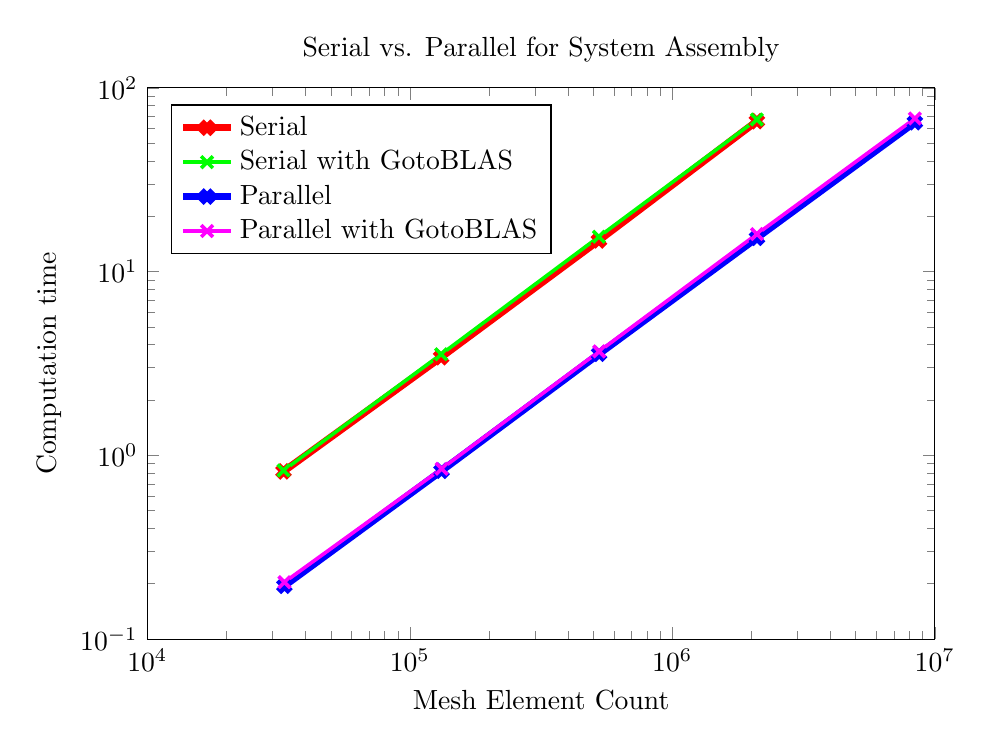
\begin{tikzpicture}

\begin{axis}[%
width=\figurewidth,
height=\figureheight,
scale only axis,
xmode=log,
xmin=10000,
xmax=10000000,
xtick={10000,100000,1000000,10000000},
xminorticks=true,
minor x tick num={3},
xlabel={Mesh Element Count},
ymode=log,
ymin=0.1,
ymax=100,
ytick={0.1,1,10,100},
yminorticks=true,
minor y tick num={3},
ylabel={Computation time},
title={Serial vs. Parallel for System Assembly},
axis on top,
legend style={at={(0.03,0.97)},anchor=north west,draw=black,fill=white,legend cell align=left}
]
\addplot [
color=red,
solid,
line width=2.6pt,
mark size=3.0pt,
mark=x,
mark options={solid}
]
table[row sep=crcr]{
33025 0.817531\\
131585 3.41866\\
525313 14.7845\\
2099201 65.8931\\
};
\addlegendentry{Serial};

\addplot [
color=green,
solid,
line width=1.3pt,
mark size=3.0pt,
mark=x,
mark options={solid}
]
table[row sep=crcr]{
33025 0.827823\\
131585 3.54683\\
525313 15.4809\\
2099201 67.2637\\
};
\addlegendentry{Serial with GotoBLAS};

\addplot [
color=blue,
solid,
line width=2.6pt,
mark size=3.0pt,
mark=x,
mark options={solid}
]
table[row sep=crcr]{
33284 0.195\\
132100 0.824\\
526340 3.57\\
2101252 15.27\\
8396804 65\\
};
\addlegendentry{Parallel};

\addplot [
color=mycolor1,
solid,
line width=1.3pt,
mark size=3.0pt,
mark=x,
mark options={solid}
]
table[row sep=crcr]{
33284 0.204\\
132100 0.845\\
526340 3.68\\
2101252 16.01\\
8396804 68.1\\
};
\addlegendentry{Parallel with GotoBLAS};

\end{axis}
\end{tikzpicture}%
      \caption{Compute times to perform system assembly.}
      \label{fig:assembly}
\end{figure}
\begin{figure}[H]
      \centering
      \setlength\figureheight{7cm}
      \setlength\figurewidth{10cm}
      % This file was created by matlab2tikz v0.4.0.
% Copyright (c) 2008--2013, Nico Schlömer <nico.schloemer@gmail.com>
% All rights reserved.
% 
% The latest updates can be retrieved from
%   http://www.mathworks.com/matlabcentral/fileexchange/22022-matlab2tikz
% where you can also make suggestions and rate matlab2tikz.
% 
% 
% 

% defining custom colors
\definecolor{mycolor1}{rgb}{1,0,1}%

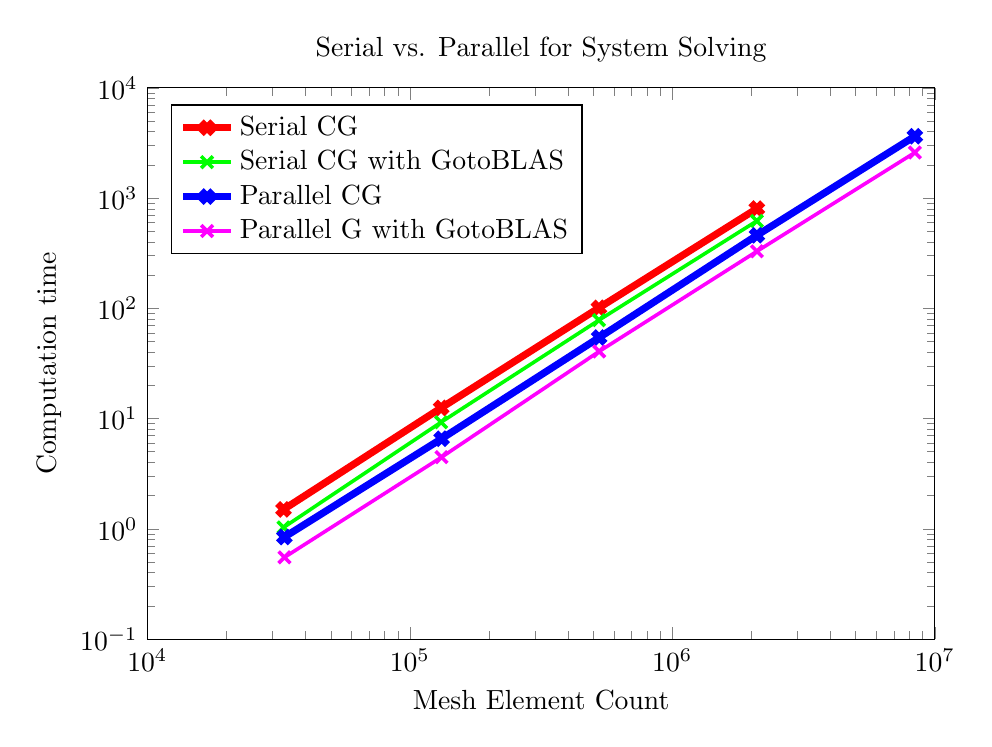
\begin{tikzpicture}

\begin{axis}[%
width=\figurewidth,
height=\figureheight,
scale only axis,
xmode=log,
xmin=10000,
xmax=10000000,
xtick={10000,100000,1000000,10000000},
xminorticks=true,
minor x tick num={3},
xlabel={Mesh Element Count},
ymode=log,
ymin=0.1,
ymax=10000,
ytick={0.1,1,10,100,1000,10000},
yminorticks=true,
minor y tick num={3},
ylabel={Computation time},
title={Serial vs. Parallel for System Solving},
axis on top,
legend style={at={(0.03,0.97)},anchor=north west,draw=black,fill=white,legend cell align=left}
]
\addplot [
color=red,
solid,
line width=2.6pt,
mark size=3.0pt,
mark=x,
mark options={solid}
]
table[row sep=crcr]{
33025 1.49912\\
131585 12.4984\\
525313 101.033\\
2099201 802.526\\
};
\addlegendentry{Serial CG};

\addplot [
color=green,
solid,
line width=1.3pt,
mark size=3.0pt,
mark=x,
mark options={solid}
]
table[row sep=crcr]{
33025 1.02973\\
131585 9.27832\\
525313 78.1647\\
2099201 620.832\\
};
\addlegendentry{Serial CG with GotoBLAS};

\addplot [
color=blue,
solid,
line width=2.6pt,
mark size=3.0pt,
mark=x,
mark options={solid}
]
table[row sep=crcr]{
33284 0.8422\\
132100 6.5692\\
526340 54.327\\
2101252 459.899\\
8396804 3641.48\\
};
\addlegendentry{Parallel CG};

\addplot [
color=mycolor1,
solid,
line width=1.3pt,
mark size=3.0pt,
mark=x,
mark options={solid}
]
table[row sep=crcr]{
33284 0.551\\
132100 4.468\\
526340 40.657\\
2101252 329.28\\
8396804 2589.78\\
};
\addlegendentry{Parallel G with GotoBLAS};

\end{axis}
\end{tikzpicture}%
      \caption{Compute times to perform system assembly.}
      \label{fig:solver}
\end{figure}
